\documentclass[conference]{IEEEtran}

\IEEEoverridecommandlockouts

\usepackage[T1]{fontenc}
\usepackage{cite}
\usepackage{amsmath,amssymb}
\usepackage{booktabs}
\usepackage{graphicx}
\usepackage{array}
\usepackage{tabularx}
\usepackage{multirow}
\usepackage{xcolor}
\usepackage{tikz}
\usepackage{url}
\usepackage{balance}
\usetikzlibrary{arrows.meta,positioning}

\newcolumntype{Y}{>{\raggedright\arraybackslash}X}
\newcolumntype{P}[1]{>{\raggedright\arraybackslash}p{#1}}

\newcommand{\toolone}{T0}
\newcommand{\tooltwo}{T1}
\newcommand{\magma}{Magma}

\title{\magma: Low-Pressure Thermoplastic Injection Into FFF-Printed Molds on a Tool-Changing Desktop Printer}

\author{
\IEEEauthorblockN{Brian Machado\IEEEauthorrefmark{1},
Clayton Haight\IEEEauthorrefmark{2},
Ethan Childerhose\IEEEauthorrefmark{3}, and
Samuel Sun\IEEEauthorrefmark{3}}
\IEEEauthorblockA{\IEEEauthorrefmark{1}Bracket Bot Research, San Francisco, CA, USA, brian@bracketbot.com}
\IEEEauthorblockA{\IEEEauthorrefmark{2}sunday.ai, Mountain View, CA, USA}
\IEEEauthorblockA{\IEEEauthorrefmark{3}Steinmetz Motors, San Francisco, CA, USA}
}

\begin{document}
\maketitle

\begin{abstract}
This paper presents \magma, a hybrid desktop manufacturing workflow in which a tool-changing fused filament fabrication (FFF) printer first fabricates a thermoplastic mold and then uses a second heated toolhead as a low-pressure melt delivery system. The process is not a replacement for industrial injection molding: it has no clamp force, no packing-pressure control, and limited thermal authority. Its value is instead in rapid, machine-local iteration on molded geometry, ports, materials, and slicer planning. The central software idea is to represent the molded part as a non-printing injected volume, separate from the printable mold bodies and the injection port. A post-processor and an experimental LavaSlicer integration use this role information to suppress the injected body from ordinary slicing, compute the injected volume, choose an injection location, and emit a controlled tool-change, heating, plunge, extrusion, dwell, and retract sequence. Generated G-code is verified across same-tool, two-tool, stationary, and rising-Z cases before physical fill quality is claimed. Pilot open-cavity trials motivate the dominant failure labels: port blockage, premature freezing, leakage, mold softening, and unsafe approach geometry. We describe the process model, slicer implementation, validation protocol, and safety constraints needed to turn the concept into a repeatable manufacturing mode.
\end{abstract}

\begin{IEEEkeywords}
additive manufacturing, fused filament fabrication, injection molding, rapid tooling, slicer software, tool-changing printers
\end{IEEEkeywords}

\section{Introduction}
Fused filament fabrication (FFF) is widely used for rapid iteration because it can convert a digital model into a physical object without dedicated tooling. Its printed parts, however, inherit layer-wise bead geometry, raster-dependent material histories, and anisotropic mechanical behavior \cite{dizonMechanical}. Injection molding can produce dense thermoplastic parts with continuous melt flow and high-quality surfaces, but it normally requires rigid tooling, clamping, and a dedicated press. Rapid tooling research has already shown the value of additively manufactured molds for short-run injection molding \cite{dizonMolds,dizonTechnologies}. The remaining question explored here is whether the printer itself can close part of that loop: print a small mold and then use another printer toolhead to fill it with molten polymer.

\magma\ investigates that middle ground. The target platform is a multi-tool desktop FFF printer, such as a Prusa XL-style tool-changing machine with independent parked hotends \cite{prusaXL}. One tool prints the mold. A second tool, typically with a larger nozzle and a different material, is heated and moved to an injection port after the mold print completes. The printer then extrudes a calculated filament length corresponding to the desired molded volume.

The contribution is not a high-pressure injection mechanism. A desktop hotend cannot reproduce the pressure, packing, cooling, or mold stiffness of an industrial press. Instead, this work contributes:
\begin{itemize}
\item a role-based CAD and slicer model that separates printable mold geometry from non-printing injected volume and port geometry;
\item a volume-to-extrusion planner for low-pressure molded deposition on an existing tool-changing FFF motion system;
\item two software paths: a G-code post-processor for fast experiments and a native LavaSlicer prototype integrated into Orca/Prusa-style slicing structures;
\item verification artifacts showing bounded injection G-code for same-tool, two-tool, stationary, and rising-Z fills;
\item an experimental protocol and failure taxonomy for evaluating fill reliability before claiming mechanical equivalence to molded parts.
\end{itemize}

\section{Related Work and Gap}
Additive manufacturing terminology and process categories are standardized in ISO/ASTM 52900 \cite{iso52900}. Within material-extrusion AM, prior work has extensively documented how process settings and build orientation affect polymer properties \cite{dizonMechanical}. This motivates hybrid routes when the target property or surface quality is closer to molded plastic than to layer-wise deposition.

Rapid tooling for injection molding is also well studied. Printed molds and inserts can reduce lead time and cost for prototype or low-volume molding, but the mold is typically transferred to a separate injection machine \cite{dizonMolds,dizonTechnologies,gohnMoldInserts,simpsonAMTool}. That separation preserves clamp force, injection pressure, and process monitoring, but it removes the immediacy of printing a mold, changing a port, and trying the next fill on the same machine. Prior work also shows that polymer tooling can deform or fail under injection loads, motivating explicit monitoring of tool strain, pressure, and thermal state \cite{gohnMoldInserts,krizsmaMonitoring}. In contrast, \magma\ keeps the printed mold on the printer build plate; the same motion system becomes a controlled melt-delivery stage. That shifts the problem from mold-insert fabrication alone to coupled CAD-role, slicer-state, tool-change, and thermal planning.

Tool-changing FFF printers create a different opportunity. They already provide multiple heated nozzles, controlled tool parking, repeatable XY positioning, and slicer-managed tool changes. \magma\ deliberately trades away the force and instrumentation of a press in exchange for machine-local iteration. Current slicers such as PrusaSlicer and OrcaSlicer are built around path generation for printed volumes \cite{prusaslicer,orcaslicer}. They do not normally treat one CAD body as a volume to be injected after the print rather than as geometry to be printed. \magma\ addresses this slicer-semantics gap.

The gap addressed here is therefore not printed tooling by itself. It is the missing CAD role model, slicer state, and machine-plan representation needed for a tool-changing printer to build the mold, suppress the injected body from ordinary slicing, and then execute a bounded low-pressure injection operation with explicit safety checks.

\section{Process Model}
Fig.~\ref{fig:concept} shows the process concept. The workflow has two stages. In the mold stage, ordinary FFF toolpaths build the mold walls, floor, port features, and any fixtures. In the injection stage, the printer performs a non-standard extrusion operation into the completed mold.

\begin{figure}[b]
\centering
\resizebox{0.96\columnwidth}{!}{%
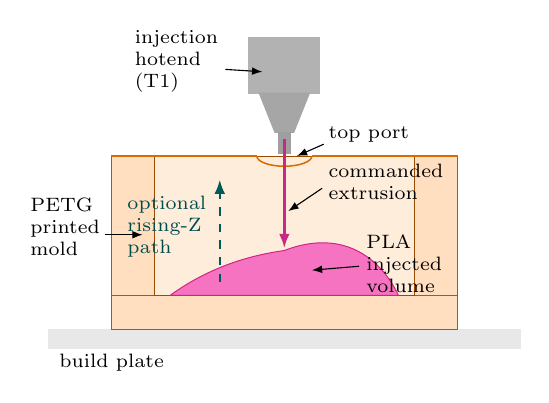
\begin{tikzpicture}[
  font=\scriptsize,
  arrow/.style={-{Latex[length=1.8mm]}, thick},
  labelarrow/.style={-{Latex[length=1.3mm]}, thin},
  mat/.style={draw, line width=0.35pt},
  note/.style={align=left, inner sep=1pt}
]
\fill[gray!18, mat] (0,0) rectangle (6.0,0.25);
\node[note, anchor=west] at (0.1,-0.18) {build plate};

\fill[orange!25, mat, draw=orange!70!black] (0.8,0.25) rectangle (5.2,0.68);
\fill[orange!25, mat, draw=orange!70!black] (0.8,0.68) rectangle (1.35,2.45);
\fill[orange!25, mat, draw=orange!70!black] (4.65,0.68) rectangle (5.2,2.45);
\fill[orange!14, draw=orange!60!black, line width=0.25pt] (1.35,0.68) rectangle (4.65,2.45);
\draw[orange!85!black, line width=0.55pt] (0.8,2.45) -- (2.65,2.45);
\draw[orange!85!black, line width=0.55pt] (3.35,2.45) -- (5.2,2.45);
\draw[orange!85!black, line width=0.55pt] (2.65,2.45) arc[start angle=180,end angle=360,x radius=0.35,y radius=0.13];
\node[note, anchor=east] at (0.7,1.55) {PETG\\printed\\mold};
\draw[labelarrow] (0.72,1.45) -- (1.2,1.45);

\fill[magenta!55, draw=magenta!85!black, line width=0.35pt]
  (1.55,0.68) .. controls (2.1,1.08) and (2.65,1.20) .. (3.0,1.25)
  .. controls (3.7,1.52) and (4.2,1.20) .. (4.45,0.68) -- cycle;
\node[note, anchor=west] at (4.0,1.08) {PLA\\injected\\volume};
\draw[labelarrow] (3.95,1.05) -- (3.35,1.0);

\fill[gray!60, mat] (2.55,3.25) rectangle (3.45,3.95);
\fill[gray!70, mat] (2.68,3.25) -- (3.32,3.25) -- (3.12,2.75) -- (2.88,2.75) -- cycle;
\fill[gray!75] (2.92,2.75) rectangle (3.08,2.48);
\node[note, anchor=east] at (2.2,3.65) {injection\\hotend\\(\tooltwo)};
\draw[labelarrow] (2.25,3.55) -- (2.72,3.52);

\draw[arrow, magenta!80!black, line width=0.9pt] (3.0,2.66) -- (3.0,1.28);
\node[note, anchor=west] at (3.52,2.72) {top port};
\draw[labelarrow] (3.5,2.6) -- (3.16,2.45);
\node[note, anchor=west] at (3.52,2.12) {commanded\\extrusion};
\draw[labelarrow] (3.48,2.04) -- (3.05,1.75);

\draw[arrow, teal!70!black, dashed, line width=0.8pt] (2.18,0.85) -- (2.18,2.15);
\node[note, anchor=east, text=teal!60!black] at (2.05,1.55) {optional\\rising-Z\\path};
\end{tikzpicture}
}
\caption{Conceptual cross-section of the \magma\ process. A mold tool prints a PETG cavity with an open top port, and an injection tool delivers PLA into the printed mold. The dashed path indicates the later rising-Z schedule, which requires separate collision checks.}
\label{fig:concept}
\end{figure}

The process is best described as low-pressure molded deposition. The hotend provides melt delivery but not industrial injection pressure. Therefore, the first process window is governed by whether enough molten material reaches the intended cavity before freezing, leaking, deforming the mold, or exceeding the tool's melt capacity. The current working material pair is PETG for the mold and PLA for the injected material. PETG provides more thermal margin than PLA for the printed mold, while PLA offers accessible melt temperatures and reliable early extrusion behavior.

The injected filament length follows directly from the desired part volume. For filament diameter $d_f$ and target injected volume $V_i$, the ideal commanded extrusion length is
\begin{equation}
E = \frac{4 V_i}{\pi d_f^2}.
\label{eq:extrusion}
\end{equation}
The planner then applies a fill ratio or overfill multiplier, splits large extrusion lengths into firmware-safe segments, and sets feed rate from a requested volumetric flow rate. This volume-based command is a necessary but insufficient condition for fill quality: it does not guarantee that the cavity has remained open, that the melt front reached the floor, or that trapped air escaped.

\section{Role-Based CAD and Slicer Semantics}
The key modeling requirement is that not all solids in the design have the same manufacturing role. The mold bodies are printable solids. The injected part body is a process volume: it defines what should be filled but must not generate perimeters, infill, supports, or a closed cap. The port identifies where the injection nozzle should enter, and vents or overflow bodies can define controlled escape paths.

\begin{figure*}[t]
\centering
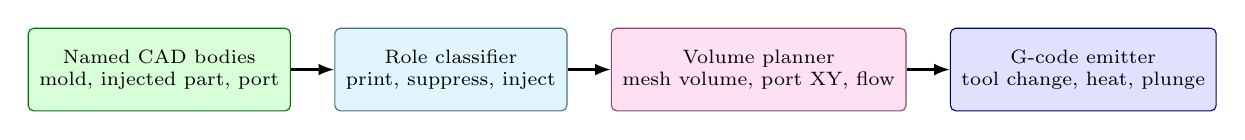
\begin{tikzpicture}[
  font=\scriptsize,
  stage/.style={draw, rounded corners=2pt, align=center, minimum width=2.8cm, minimum height=1.05cm, inner sep=4pt},
  arrow/.style={-{Latex[length=2mm]}, thick}
]
\node[stage, fill=green!15, draw=green!45!black] (cad) {Named CAD bodies\\mold, injected part, port};
\node[stage, fill=cyan!12, draw=cyan!45!black, right=0.55cm of cad] (roles) {Role classifier\\print, suppress, inject};
\node[stage, fill=magenta!12, draw=magenta!50!black, right=0.55cm of roles] (plan) {Volume planner\\mesh volume, port XY, flow};
\node[stage, fill=blue!12, draw=blue!45!black, right=0.55cm of plan] (gcode) {G-code emitter\\tool change, heat, plunge};
\draw[arrow] (cad) -- (roles);
\draw[arrow] (roles) -- (plan);
\draw[arrow] (plan) -- (gcode);
\end{tikzpicture}
\caption{Role-aware slicer pipeline. Named CAD bodies are classified into printable mold geometry, non-printing injected volume, and port or vent features. The injected body drives volume calculation and G-code generation while being suppressed from ordinary FFF toolpath generation.}
\label{fig:pipeline}
\end{figure*}

Fig.~\ref{fig:pipeline} summarizes the intended pipeline. A slicer that treats every solid as printable can accidentally close the port, fill the cavity with support, or print the injected part as ordinary FFF geometry. A \magma-compatible slicer must instead preserve role information through import, arrangement, slicing, preview, and G-code export.

\begin{figure}[t]
\centering
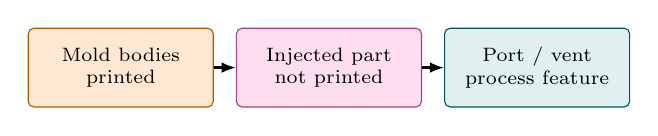
\begin{tikzpicture}[
  font=\scriptsize,
  role/.style={draw, rounded corners=2pt, align=center, minimum width=2.35cm, minimum height=1.0cm, inner sep=4pt}
]
\node[role, fill=orange!18, draw=orange!70!black] (mold) {Mold bodies\\printed};
\node[role, fill=magenta!13, draw=magenta!65!black, right=0.28cm of mold] (part) {Injected part\\not printed};
\node[role, fill=teal!12, draw=teal!65!black, right=0.28cm of part] (port) {Port / vent\\process feature};
\draw[-{Latex[length=1.8mm]}, thick] (mold) -- (part);
\draw[-{Latex[length=1.8mm]}, thick] (part) -- (port);
\end{tikzpicture}
\caption{Required model roles. Mold bodies are printed. The injected part body and injection-port marker are non-printing process geometry that guide volume calculation and nozzle placement.}
\label{fig:roles}
\end{figure}

\section{Software Implementation}
\subsection{Phase 0 Post-Processor}
The first implementation is the \texttt{magma\_inject.py} post-processor. It takes sliced mold G-code, optionally a mold STL, and writes a new G-code file with an injection block inserted before the printer's end sequence. The script can estimate a blind pocket from G-code by rasterizing extrusion paths, flood-filling enclosed empty regions, and measuring the largest cavity across layers. Alternatively, it can use STL geometry by finding the largest up-facing interior floor below the rim. The estimated cavity centroid becomes the injection XY location, and the cavity volume sets the extrusion length through (\ref{eq:extrusion}).

The generated block switches to relative extrusion, performs the tool change when the injection tool differs from the mold tool, waits for the injection temperature, travels to the port, plunges below the rim, primes, injects the computed volume in segmented extrusion moves, dwells, retracts, and lifts clear. The script also handles practical tool-changing details such as registering an otherwise unused Prusa XL tool at startup and patching filament-use metadata so the printer and preview recognize the second tool.

\subsection{Native LavaSlicer Prototype}
The post-processor is useful for experiments, but it is brittle because it relies on conventions in the already-generated G-code. The native LavaSlicer/PrusaSlicer prototype integrates the same concept earlier in the slicing pipeline. Fig.~\ref{fig:settings} shows the new Injection settings section exposed in the slicer UI. It makes injection enable, injected-body name, temperature, bed-temperature override, tool selection, fill ratio, and plunge depth explicit slicer state rather than hidden custom end code. Additional expert settings cover port name, manual or model-derived XYZ target, start and end Z, volume, flow, and dwell.

\begin{figure}[t]
\centering
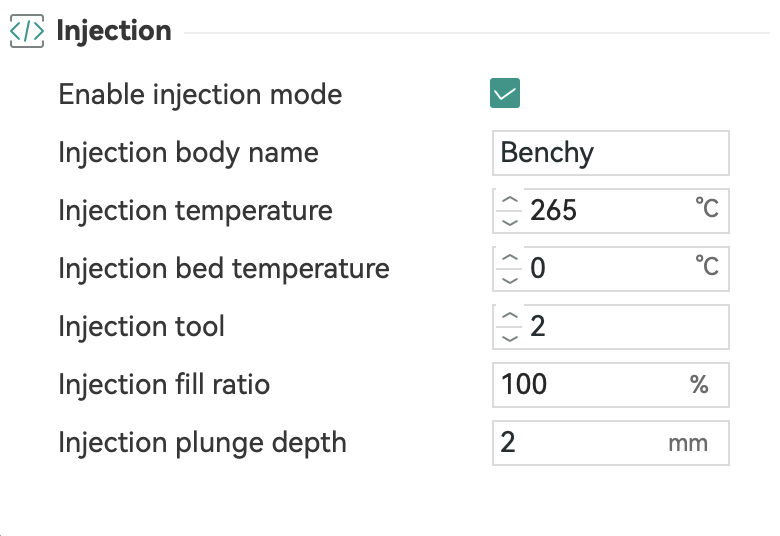
\includegraphics[width=0.82\columnwidth]{figures/injection_settings_panel.png}
\caption{Prototype LavaSlicer Injection settings panel. The controls expose injected-body name, injection temperature, bed-temperature override, tool index, fill ratio, and plunge depth as slicer state.}
\label{fig:settings}
\end{figure}

When injection mode is enabled, the slicer identifies helper geometry by object or volume name and filters the injected part and port marker out of the volumes passed to ordinary slicing. During G-code generation, the prototype accumulates transformed mesh volume from all matching injected-part helpers, finds the port helper when present, otherwise falls back to the injected body's top-center, and appends a tagged custom extrusion sequence. The tagged sequence makes the injection operation visible to the G-code processor and preview instead of hiding it inside end code.

For repeatable experiments, the planner must make seven states explicit: injected volume, injection point, selected injection tool, temperature, fill ratio, plunge depth, and volumetric-flow limit. The current prototype exposes these values as settings or derives them from the injection body and filament profile. Guard checks reject invalid extruder indices, zero volume or flow, descending start/end Z, and manual pour points outside the bed.

\section{G-code Verification}
Before treating \magma\ as a physical manufacturing process, the software output was checked as a machine plan. Table~\ref{tab:gcodeverify} summarizes representative G-code artifacts generated by the post-processor and by the native LavaSlicer prototype. A companion parser regenerates the table values from the G-code comments and extrusion moves, including temperature waits, segment counts, tool path, and commanded extrusion length. These checks verify that the planner produces volume-derived extrusion commands, splits them into bounded moves, and surrounds them with the required heat-wait, tool-change, plunge, dwell, retract, and lift sequence. They do not prove that a cavity fills completely; they verify that the machine is commanded to perform the intended injection operation.

\begin{table*}[t]
\caption{Representative G-code Verification Artifacts}
\label{tab:gcodeverify}
\centering
\scriptsize
\setlength{\tabcolsep}{3.1pt}
\begin{tabularx}{\textwidth}{@{}P{0.14\textwidth}P{0.15\textwidth}P{0.12\textwidth}P{0.14\textwidth}P{0.14\textwidth}Y@{}}
\toprule
Artifact & Implementation path & Injection command & Thermal/flow command & Segmentation & Verified sequence \\
\midrule
Tiny cube & Hand-authored Phase 0 block & 1000 mm$^3$ & 240$^\circ$C, 15 mm$^3$/s & 10 $\times$ 41.575 mm & Relative extrusion, heat wait, center approach, 2 mm plunge, dwell, retract, and lift. \\
Mold2 pocket & Phase 0 cavity estimate & 712 mm$^3$ & 230$^\circ$C, 25 mm$^3$/s & 2 $\times$ 148.008 mm & Mold tool unload and cool, \toolone$\rightarrow$\tooltwo\ change, injection-tool heat wait, 2 mm plunge. \\
Cube pocket & Phase 0 cavity estimate & 936 mm$^3$ & 240$^\circ$C, 25 mm$^3$/s & 3 $\times$ 129.722 mm & Same-tool injection path with explicit heat wait, port travel, 2 mm plunge, dwell, retract, and lift. \\
10 mm part helper & Native LavaSlicer & 0.55 cm$^3$ & 260/265$^\circ$C, 4 mm$^3$/s & 45 $\times$ 5 mm + 1.37 mm & Typed injection-pour layer, model-helper part source, top-center fallback port, \toolone$\rightarrow$\tooltwo\ change. \\
30 mm port helper & Native LavaSlicer & 27.0 cm$^3$ & 260/275$^\circ$C, 48.1 mm$^3$/s & 2244 $\times$ 5 mm + 4.82 mm & Named part and port sources, rising-Z schedule from 3.0 to 31.5 mm, \toolone$\rightarrow$\tooltwo\ change. \\
\bottomrule
\end{tabularx}
\end{table*}

The verification cases exercise two different sources of injected volume. The Phase 0 post-processor appends an injection block after ordinary mold G-code and can operate from either a hand-specified target volume or an estimated pocket. The native prototype emits an explicit \texttt{Injection pour} layer whose comments retain the source of the injected part and the source of the port. This distinction matters because a native slicer can present the injection operation as first-class process geometry in preview, whereas the post-processor can only append and annotate a block after slicing.

The native rising-Z artifact is intentionally a software stress case rather than a recommended first physical trial. It demonstrates that the slicer can generate thousands of small, bounded extrusion moves while advancing the nozzle from the lower cavity toward the top of the part. Whether that strategy is physically safe depends on collision checking, venting, and mold stiffness, so it is carried into the validation plan as a hypothesis rather than a result.

The accompanying package reinforces this distinction by regenerating the G-code verification table, checking the cited slicer-source hooks, rendering the PDF, and reporting absent fill-trial measurements as an explicit audit warning.

\section{Experimental Method}
The validation path should begin with geometries that expose failure modes rather than hide them. The initial setup session therefore used simple cup-like open cavities rather than complex closed shapes, so that the first question was material delivery rather than part complexity. The current test article is a 10 mm-scale open cup, cylinder, or block cavity printed in PETG and filled with PLA from a larger injection nozzle. This geometry is simple enough to measure visually and by mass, yet large enough to reveal freezing, port blockage, leakage, and mold softening.

\begin{table}[t]
\caption{Initial Experimental Configuration}
\label{tab:config}
\centering
\scriptsize
\setlength{\tabcolsep}{2.2pt}
\begin{tabularx}{\columnwidth}{@{}p{0.27\columnwidth}p{0.30\columnwidth}Y@{}}
\toprule
Parameter & Current value & Purpose \\
\midrule
Mold tool/material & \toolone, 0.4 mm, PETG & Accurate cavity and thermal margin \\
Injection tool/material & \tooltwo, 0.8 mm, PLA & Larger outlet and lower melt temperature \\
Geometry & 10 mm cup or cube cavity & Fast iteration and interpretable failures \\
Injection command & Mesh or cavity volume & Relate commanded extrusion to part volume \\
Initial sweep & 240--275$^\circ$C, 10--30 mm$^3$/s & Map the fill window before complex molds \\
\bottomrule
\end{tabularx}
\end{table}

The trial sequence used for the first tests is:
\begin{enumerate}
\item print the PETG mold with a real, open port into the cavity;
\item heat, pick, and optionally purge the PLA injection tool;
\item approach a circular top port at a collision-safe height;
\item plunge by a bounded distance below the rim;
\item extrude the calculated volume at a controlled volumetric flow rate;
\item record commanded volume, delivered mass change, visible fill depth, leakage, port blockage, mold deformation, nozzle contamination, and removal quality.
\end{enumerate}

\section{Preliminary Observations}
The current hardware and software trials support a limited feasibility claim: custom G-code can print a small mold-like cavity and then deliver molten polymer through a second tool. In the initial session, material visibly exited the injection tool and entered the test geometry, but the result was not yet a controlled, fully packed molded part. Some early parts showed messy deposition and incomplete lower-cavity fill, which is consistent with the expected low-pressure and rapid-cooling limits.

These observations are included to motivate the validation protocol and failure taxonomy; they are not treated as a quantitative fill-reliability result.

The trials also show why a naive top-pour sequence is not enough for a robust process. Melt can freeze against the mold before filling the lower cavity, especially when commanded flow is slow or nozzle temperature is too low. Conversely, one early G-code path attempted to inject too quickly; the printer effectively limited or rejected the requested extrusion rather than delivering the intended volume. This makes volumetric-flow limiting a first-class process constraint, not a tuning detail.

Tool-changing behavior is also process-critical. A parked injection tool may sit near a standby temperature, observed around 180$^\circ$C in early testing, and may not be ready when selected unless the G-code explicitly waits for injection temperature. Startup G-code must register tools that are not used during the mold print but are needed later for injection. Purge and wipe behavior matters because residue on the injection nozzle can prevent clean seating at the port; in the observed setup, cleaning and purging had to be managed explicitly rather than assumed as a background printer function.

Finally, the printer's tool-changing geometry constrains the injection path. The Prusa XL-style dock and toolhead envelope allow lateral tool changes but make deep vertical approaches risky near printed mold walls, adjacent docks, and calibration structures. For this reason, the injection planner must treat plunge depth and port location as collision-checked motion, not merely as scalar process settings.

\begin{figure}[t]
\centering
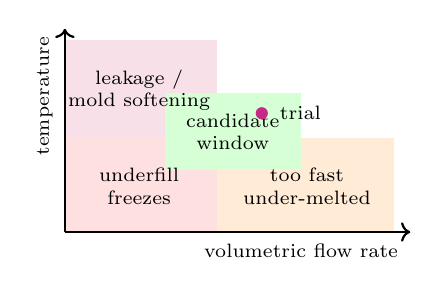
\begin{tikzpicture}[font=\scriptsize, x=0.82cm, y=0.58cm]
\fill[red!12] (0,0) rectangle (2.35,2.05);
\fill[orange!16] (2.35,0) rectangle (5.1,2.05);
\fill[purple!12] (0,2.05) rectangle (2.35,4.2);
\fill[green!16] (1.55,1.35) rectangle (3.65,3.05);
\draw[->, thick] (0,0) -- (5.35,0) node[below left=1pt] {volumetric flow rate};
\draw[->, thick] (0,0) -- (0,4.45) node[above left=1pt, rotate=90] {temperature};
\node[align=center] at (1.15,1.0) {underfill\\freezes};
\node[align=center] at (3.75,1.0) {too fast\\under-melted};
\node[align=center] at (1.15,3.1) {leakage /\\mold softening};
\node[align=center] at (2.6,2.2) {candidate\\window};
\fill[magenta!80!black] (3.05,2.6) circle (2.2pt);
\node[anchor=west] at (3.18,2.6) {trial};
\end{tikzpicture}
\caption{Qualitative process window. Reliable filling requires enough temperature and flow to reach the bottom of the cavity without exceeding hotend melting capacity, blocking the port, leaking, or softening the printed mold.}
\label{fig:window}
\end{figure}

Fig.~\ref{fig:window} gives the working failure taxonomy. The next measured dataset should assign each trial one or more failure labels so that process changes can be compared without relying on subjective print impressions.

\section{Validation Plan}
The first publishable dataset should remain deliberately small. A single standardized cavity with a known port diameter is enough to test whether temperature, volumetric flow rate, port geometry, and Z schedule change fill completeness. More complex split molds or Benchy-derived cavities should wait until the simple dataset is interpretable.

\begin{table}[t]
\caption{Validation Matrix for a First Quantitative Dataset}
\label{tab:validation}
\centering
\scriptsize
\setlength{\tabcolsep}{2.0pt}
\begin{tabularx}{\columnwidth}{@{}p{0.23\columnwidth}p{0.24\columnwidth}p{0.25\columnwidth}Y@{}}
\toprule
Variable & Sweep & Primary metric & Failure label \\
\midrule
Nozzle temperature & 240, 255, 275$^\circ$C & Bottom fill depth & Freezing or softening \\
Flow rate & 10, 20, 30 mm$^3$/s & Delivered mass & Flow limit \\
Port geometry & Diameter, chamfer & Leakage/blockage & Port failure \\
Z schedule & Top pour, rising-Z & Void fraction & Trapped air \\
\bottomrule
\end{tabularx}
\end{table}

For each trial, the commanded injected volume should be compared against mass change using measured filament density or a calibrated filament cross-section. The cavity should be photographed from the same view, and selected trials should be sectioned to distinguish surface fill from true bottom fill. A rising-Z schedule should only be evaluated after collision checks confirm that the injection tool can enter the port without striking the mold walls.

\section{Reproducibility and Threats to Validity}
The submission package is organized so that each claim class can be checked separately. The build regenerates the manuscript PDF, rendered page images, PDF production report, claim-scope report, G-code verification table, fill-trial plan summary, fill-trial asset report, and submission manifest. The G-code table is not hand-entered; it is regenerated from representative machine files and cross-checked against native slicer source hooks. This supports the software claim that \magma\ can emit bounded, interpretable injection operations.

The physical-process claim remains weaker. The current observations come from one tool-changing printer, one PETG/PLA material pairing, and small open cavities. They do not establish pressure control, packing, repeatability, mechanical properties, or complete fill in closed molds. To avoid conflating planned commands with physical results, measured rows are not counted as publishable unless the trial CSV includes required metrics and points to existing executed G-code and photo evidence. The validation matrix in Table~\ref{tab:validation} is therefore the minimum next evidence needed to turn the present feasibility result into a controlled process result.

\section{Discussion}
\magma\ is promising because it uses capabilities already present in tool-changing FFF printers: multiple heated tools, software-controlled tool selection, accurate positioning, and slicer access to model geometry. The strongest software insight is that the injected part must be represented as process geometry rather than as printable geometry. Without that distinction, the slicer can produce a plausible preview while generating a blocked port or a filled cavity.

The process also has clear limits. It currently lacks pressure sensing, clamp force, closed-loop fill-front observation, and industrial packing control. Those omissions are more severe than in printed-tooling studies that still use injection molding presses, because here the printer hotend is both the heater and the delivery actuator. Small, open, or vented cavities are a realistic starting point; tall, thin, sealed, or poorly vented cavities are likely to fail. The mold material can soften, deform, or bond to the injected material, and the nozzle can damage the port during approach. These constraints are not incidental details: they are the core conditions that a safe slicer feature must validate.

From a software perspective, native support should add geometric validation before slicing. The slicer should verify that the injected body is inside the mold cavity, the port connects to that cavity, vents or overflow paths exist when required, and the selected tool can physically approach the port. The preview should show the mold, non-printing injected body, port, planned plunge, and injection extrusion separately from ordinary printed extrusion.

\section{Conclusion}
This paper introduced \magma, a low-pressure hybrid manufacturing workflow that prints a thermoplastic mold and then injects molten filament into it using a second tool on the same FFF printer. The current implementation demonstrates the core software path: role-based model handling, injected-volume suppression, volume-to-extrusion planning, tool-change sequencing, and verified injection G-code generation across same-tool, two-tool, stationary, and rising-Z cases. The approach should be evaluated as low-pressure molded deposition rather than industrial injection molding. The next decisive step is a compact quantitative dataset that maps the fill window and separates true cavity filling from extrusion-command success.

\balance
\begin{thebibliography}{00}
\bibitem{iso52900}
ISO/ASTM 52900:2021, ``Additive manufacturing -- General principles -- Fundamentals and vocabulary,'' International Organization for Standardization, 2021.

\bibitem{dizonMechanical}
J. R. C. Dizon, A. H. Espera, Q. Chen, and R. C. Advincula, ``Mechanical characterization of 3D-printed polymers,'' \emph{Additive Manufacturing}, vol. 20, pp. 44--67, 2018, doi: 10.1016/j.addma.2017.12.002.

\bibitem{dizonMolds}
J. R. C. Dizon, A. D. Valino, L. R. Souza, A. H. Espera, Q. Chen, and R. C. Advincula, ``Three-dimensional-printed molds and materials for injection molding and rapid tooling applications,'' \emph{MRS Communications}, vol. 9, pp. 1267--1283, 2019, doi: 10.1557/mrc.2019.147.

\bibitem{dizonTechnologies}
J. R. C. Dizon, A. D. Valino, L. R. Souza, A. H. Espera, Q. Chen, and R. C. Advincula, ``3D printed injection molds using various 3D printing technologies,'' \emph{Materials Science Forum}, vol. 1005, pp. 150--156, 2020, doi: 10.4028/www.scientific.net/MSF.1005.150.

\bibitem{gohnMoldInserts}
A. M. Gohn, D. Brown, G. Mendis, S. Forster, N. Rudd, and M. Giles, ``Mold inserts for injection molding prototype applications fabricated via material extrusion additive manufacturing,'' \emph{Additive Manufacturing}, vol. 51, Art. no. 102595, 2022, doi: 10.1016/j.addma.2022.102595.

\bibitem{simpsonAMTool}
P. Simpson, A. D. Zakula, J. Nelson, J. K. Dworshak, E. M. Johnson, and C. A. Ulven, ``Injection molding with an additive manufactured tool,'' \emph{Polymer Engineering \& Science}, vol. 59, no. 9, pp. 1911--1918, 2019, doi: 10.1002/pen.25192.

\bibitem{krizsmaMonitoring}
S. Krizsma, N. K. Kovacs, J. G. Kovacs, and A. Suplicz, ``In-situ monitoring of deformation in rapid prototyped injection molds,'' \emph{Additive Manufacturing}, vol. 42, Art. no. 102001, 2021, doi: 10.1016/j.addma.2021.102001.

\bibitem{prusaXL}
Prusa Research, ``Original Prusa XL,'' product documentation: \url{prusa3d.com/product/original-prusa-xl-5-toolhead-3d-printer/}

\bibitem{prusaslicer}
Prusa Research, ``PrusaSlicer,'' GitHub repository: \url{github.com/prusa3d/PrusaSlicer}

\bibitem{orcaslicer}
SoftFever, ``OrcaSlicer,'' GitHub repository: \url{github.com/SoftFever/OrcaSlicer}
\end{thebibliography}

\end{document}
